\documentclass[10pt,letterpaper]{article}

\usepackage[margin=0.85in]{geometry}
\usepackage{fontspec}
\defaultfontfeatures{Ligatures=TeX}
\setmainfont{texgyrepagella-regular.otf}[
  BoldFont=texgyrepagella-bold.otf,
  ItalicFont=texgyrepagella-italic.otf,
  BoldItalicFont=texgyrepagella-bolditalic.otf]
\setsansfont{texgyreheros-regular.otf}[
  BoldFont=texgyreheros-bold.otf,
  ItalicFont=texgyreheros-italic.otf,
  BoldItalicFont=texgyreheros-bolditalic.otf]
\setmonofont{lmmono10-regular.otf}

\usepackage{amsmath,amssymb}
\usepackage{graphicx,float}
\usepackage{tabularx,booktabs,array,needspace}
\usepackage{cite}
\usepackage{xcolor,xurl}
\usepackage{microtype,parskip}
\usepackage[colorlinks=true,linkcolor=teal,citecolor=teal,urlcolor=teal]{hyperref}
\usepackage{bookmark}
\usepackage{fancyhdr}

\hypersetup{
  pdftitle={Slop Ninja: Public detectors, private transformation models, and paid inference on Bittensor},
  pdfauthor={Slop Ninja Research},
  pdfsubject={Subnet design whitepaper, draft 0.6}}
\setcounter{secnumdepth}{2}
\setlength{\emergencystretch}{3em}
\renewcommand{\arraystretch}{1.15}
\newcolumntype{L}{>{\raggedright\arraybackslash}X}
\newcommand{\tightlist}{\setlength{\itemsep}{0pt}\setlength{\parskip}{0pt}}

\pagestyle{fancy}
\fancyhf{}
\fancyhead[L]{\small\sffamily Slop Ninja}
\fancyhead[R]{\small\sffamily Design draft 0.6}
\fancyfoot[C]{\small\thepage}
\setlength{\headheight}{14pt}
\widowpenalty=10000
\clubpenalty=10000
\brokenpenalty=10000

\title{Slop Ninja\\[0.5em]
  \large Public detectors, private transformation models,\\
  and paid inference on Bittensor}
\author{Slop Ninja Research}
\date{September 10, 2026\\Draft 0.6}

\begin{document}
\maketitle

\section*{Abstract}\label{abstract}

Slop Ninja proposes a Bittensor subnet launching with two tasks:
author and AI-origin detection (A), and author-directed text
transformation (B).
Miners develop private models and compete on the usefulness of their
outputs. They receive network emissions for benchmark performance and
can separately sell asynchronous inference at market prices denominated
in the subnet's alpha token. The protocol
requires no publication of model weights, feature definitions, adapters,
or training recipes.

Every customer inference request is encrypted for its assigned miner.
The customer's source text, reference writing, style profile, and
editorial brief are not automatically disclosed to validators, routing
services, or other miners. Customers receive encrypted results and may
separately provide evidence to a specific validator of their choice.
Subnet-owned benchmarks provide the authorized material that validators
need to assess accuracy and target style, with preservation, readability,
and tone as constraints on B.
Transformation miners compete against Pangram and qualified subnet
AI-origin detectors. Emission eligibility
requires bounded reciprocal service: detectors supply predictions and
transformation miners supply authorized challenge rewrites without a
per-call fee to each other. Retired benchmark rewrites feed later
detection rounds. Detector reports establish observations rather than
human authorship or preserved meaning.

On-chain contracts coordinate offers, commitments, deadlines, and
payments; miners execute inference privately off-chain. Published hash
rules determine counterpart and evidence-preparer assignments. Every scored
benchmark submission receives the required review at launch. Final
judgments require strictly more than two-thirds of frozen eligible
validator weight, assuming less than one-third is dishonest and each
signer inspects the evidence.
This draft specifies the proposed architecture, training data, reward
rules, and trust assumptions. It also reports the limits of the existing
prototype. Direct monetary use of private detector responses remains
unresolved: fixed paired credits do not guarantee conserved native
payouts. A reliable rewriting model, private inference service, and live
reward mechanism remain to be demonstrated.

\section{Purpose and scope}\label{purpose-and-scope}

A useful writing model should retain a writer's argument while allowing
changes to expression. The same person may want a passage closer to
their own voice, more accessible to a general audience, or more forceful
without becoming less accurate. An authorship model can help describe
those differences. A detector can measure one aspect of how the result
is classified. Neither measurement alone establishes that the revision
is good.

The subnet therefore evaluates three tasks separately:

\begin{enumerate}
\def\labelenumi{\arabic{enumi}.}
\tightlist
\item
  Identify authors and documented human/model production histories.
\item
  Transform writing toward a requested voice, optionally reducing
  detection by Pangram, while preserving the source's meaning and
  intended tone.
\item
  Improve writing for an explicit audience and editorial purpose.
\end{enumerate}

The evasion target is a reported AI-generated \textbf{plus AI-assisted}
fraction strictly below 10\%, with preservation and quality requirements
satisfied. Reaching zero is a desirable measured outcome, not a promise
of this design. A model-origin text retains that recorded origin after a
successful rewrite. Detector evasion does not change its production
history.

The initial scope is English prose, document-level author/origin
predictions, and bounded asynchronous editing jobs. Span-level origin
labels, multilingual rewards, and arbitrary-length manuscripts need
their own validated datasets. There is no requirement for token
streaming or interactive latency.

\section{Related subnets, services, and research}\label{related-work}

This representative survey covers direct task competitors and relevant
evaluation and inference infrastructure. It uses project-maintained
documentation and research publications checked on September 9, 2026.
Subnet numbers below follow the projects' own documentation; this is
not an independent audit of live chain state. Published service claims
are distinguished from results measured by this project.

\subsection{Bittensor precedents}\label{related-subnets}

It's AI and BitMind's GAS supply the closest task and incentive
precedents. It's AI documents human/AI text classification on SN32,
with miners serving detection requests. Its FAQ says the team does not
know which models its leading miners use. This provides a precedent for
evaluating detection endpoints with undisclosed implementations. GAS
documents an explicit competition between detection models and
generators that try to fool them~\cite{itsai,itsaifaq,bitmindgas}.

\par\medskip\noindent
\begin{tabularx}{\linewidth}{@{}>{\raggedright\arraybackslash}p{0.16\linewidth}LL@{}}
\toprule
Project & Documented approach & Relevance to Slop Ninja \\
\midrule
It's AI (SN32) & Human/AI text detection, including sentence-level
probabilities, through miner endpoints~\cite{itsai,itsaifaq} & Direct
comparison for origin detection; compare calibration and generalization
on the same independently labeled text \\
BitMind GAS (SN34) & Image/video/audio detector submissions and
image/video generator endpoints; generation rewards include fooling
detectors~\cite{bitmindgas,gasgeneration} & Direct precedent for adversarial
incentives; text revision adds source-preservation and requested-voice
constraints \\
Macrocosmos Finetuning (SN37) & Miners publish competition models on
public Hugging Face repositories for validator evaluation~\cite{finetuning} & Precedent for
rewarding model improvements through submitted weights; Slop Ninja
proposes private model serving \\
Chutes (SN64) & Serverless model inference and metered service, with
documented confidential-serving options~\cite{chutes,chutesprivacy} &
Paid inference and private serving infrastructure; writing quality
requires separate task evaluation \\
Targon (SN4) & Managed compute and inference; confidential VMs with
attestation-bound key release for proprietary
workloads~\cite{targon,targonconfidential} & Hardware-based endpoint
protection and private-model execution are established design topics \\
\bottomrule
\end{tabularx}
\par\medskip

These projects establish that detection competition, adversarial
generation, language-model training rewards, and paid private inference
already have Bittensor precedents. Their documented mechanisms evaluate
different properties. For example, GAS requires submitted detector
weights, whereas Slop Ninja permits private detector services. Chutes
documents confidential serving and request/response encryption, and
Targon describes hardware attestation and key release.
Those hardware assumptions differ from this paper's default trust in
the assigned miner after decryption. A secure execution environment
alone does not establish that a revision preserved an argument.

\subsection{Existing writing services}\label{related-services}

Pangram and GPTZero already offer human/model-origin classification,
including mixed or assisted categories. Pangram is the required
external opponent here; GPTZero is another useful comparison on
rights-cleared benchmark material. Their output categories and scores
must be mapped explicitly to the evaluation's documented production
labels. Agreement among detectors does not establish an author's
identity~\cite{pangramcard,gptzero}.

Grammarly documents personal voice profiles and a feature for rewriting
in the user's voice. Wordtune offers sentence and paragraph rewriting,
formality changes, shortening, and expansion. QuillBot documents
multiple paraphrasing modes, including custom and Humanizer modes, and
warns that its Creative mode can alter meaning. These are direct
comparators for author-directed revision and writing improvement;
personalization and editorial controls are existing product
capabilities~\cite{grammarlyvoice,wordtune,quillbot}.

Undetectable AI explicitly markets humanization modes intended to
bypass detectors. That documents an existing commercial objective;
this survey does not independently establish its bypass or preservation
performance~\cite{undetectable}. Comparing such services requires the
same sources, briefs, retained outputs, and blinded preservation review
used for subnet miners. A product's advertised detector score cannot
substitute for that comparison. Hosted service comparisons use
authorized benchmark text and do not create an exception to confidential
customer delivery.

\subsection{Research foundations and proposed contribution}\label{related-research}

Gero et al. model style through controls over function-word frequencies
and syntactic constructions while retaining content words. This is a
direct antecedent for combining lexical and grammatical features.
StyleRemix uses interpretable style axes and LoRA modules for authorship
obfuscation, providing a relevant comparison for controllable
rewriting~\cite{linguisticcontrols,styleremix}. Authorship obfuscation
changes evidence available to an author classifier; matching a requested
writer and preserving every required claim remain separate evaluation
questions.

The PAN/ELOQUENT 2024 task paired human/AI detection with generation and
obfuscation intended to avoid it, offering a prior benchmark for an
adversarial loop. DIPPER demonstrated paraphrase attacks on several
then-current detectors and studied a retrieval-based defense. Those
results motivate adaptive opponents and held-out evaluation; they do
not establish performance against Pangram 4 or Slop Ninja's future
incumbents~\cite{pan2024,dipper}.

The proposed contribution is a text-focused protocol connecting
origin-detection competition to author-directed transformation, with
independent preservation review and a separate writing-improvement
reward. Transformation miners face both Pangram and the best eligible
subnet detector; retired, authorized rewrites train and test later
detectors. Miners retain their models and can sell jobs through an
alpha-denominated market with explicit recipient encryption. This
combination requires validation against the precedents above. The
survey establishes neither uniqueness across all subnets nor superior
performance by an implementation that has not yet been built.

\section{Participants and the two kinds of
work}\label{participants-and-the-two-kinds-of-work}

Miners register signed service endpoints and capabilities and retain
their models. Customers buy detection and transformation jobs through
separately quoted offers. Validators evaluate subnet-owned
benchmark tasks and submit weights. Benchmark curators maintain
permitted source material, production records, and hidden evaluation
labels. A customer-facing gateway may relay ciphertext, but receives no
decryption key.

Benchmark operator and coordinator denote administrative duties assigned
to named curators and validators before each round: funding and managing
the round, recording protocol-derived assignments, and obtaining baseline evidence. A pilot may
combine these duties in one service. The task owner is the customer for
private inference and the curator for a benchmark. Authorized evaluators
and auditors are assigned validators; judges, readers, and authorized
reviewers perform independent review for those validators. Automated
judges require the qualification described in
Section~\ref{preservation-before-revision-rewards}. The settlement adapter
is the proposed contract software for customer escrow and alpha
transfers, described in
Section~\ref{paid-asynchronous-jobs-and-on-chain-coordination}.

\par\medskip\noindent
\begin{tabularx}{\linewidth}{@{}LLL@{}}
\toprule
Property & Customer inference & Subnet benchmark \\
\midrule
Purpose & Serve a customer's request & Measure miners for emissions \\
Launch services & A: detection; B: transformation & A: detection;
B: transformation \\
Source of text & Customer & Authorized benchmark collection \\
Default input recipients & Customer and assigned miner & Curator,
assigned service miners, validators, commissioned reviewers \\
Evaluation & Customer acceptance & Fixed scoring policy and independent
review \\
Pangram submission & Excluded from the confidential job protocol &
Required for evasion tasks \\
Payment & Customer's quoted fee & Performance-dependent emissions \\
Training reuse & No automatic reuse & Only under the collection's
release terms \\
\bottomrule
\end{tabularx}
\par\medskip

\begin{figure}[H]
\centering
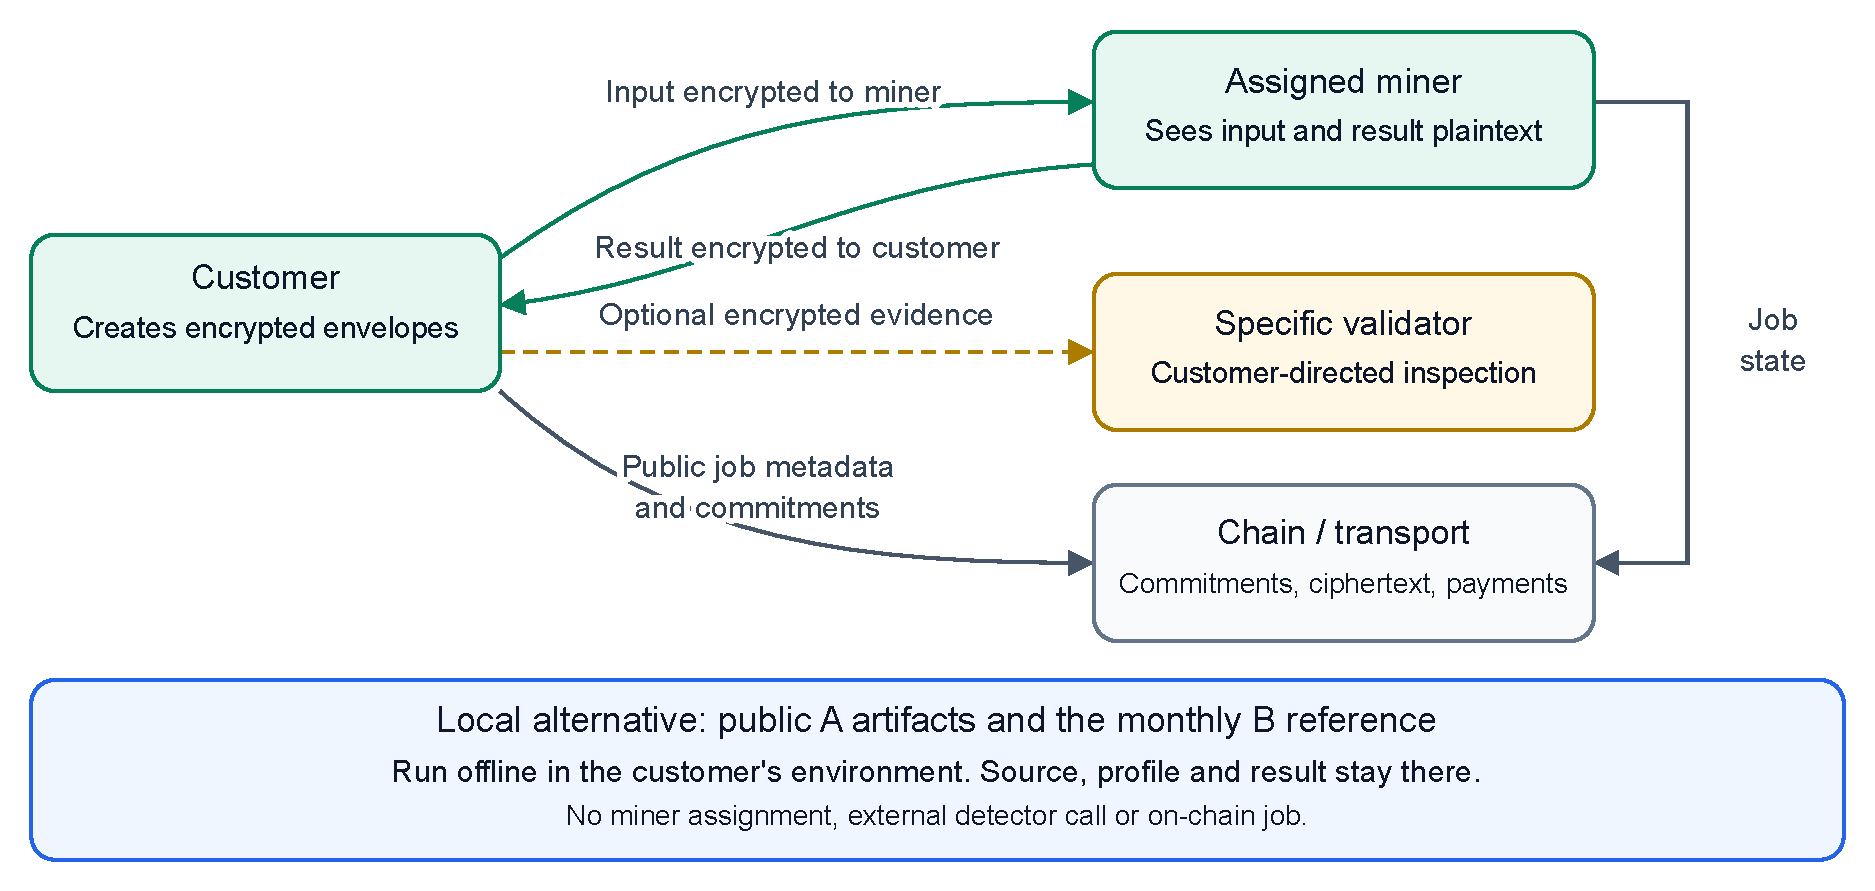
\includegraphics[width=\linewidth]{figures/private-inference.pdf}
\caption{Customer inference and optional evidence disclosure. Only the
addressed recipient can decrypt each envelope; endpoint handling remains
a trust assumption.}
\end{figure}

Customer tasks do not become benchmark examples automatically.
Validators must not obtain customer inputs through an audit exception, a
shared support key, or an arbitration process. A customer may initiate a
separate, explicitly addressed evidence disclosure as described in
Section~\ref{customer-directed-evidence-disclosure}. This applies to both
detection and transformation requests. An author's uploaded reference collection can be more identifying
than the query itself and receives the same protection.

Miners may advertise specialties, prices, length limits, and delivery
times. The network evaluates their observable service performance. It
cannot infer how many GPU hours they used, whether they own every
component, or which private weights produced a response. Emissions
create an incentive to improve training; they do not reimburse
unverifiable training claims.

\section{Model interfaces and starter
architectures}\label{model-interfaces-and-starter-architectures}

The two launch interfaces, A for detection and B for transformation,
define compatible jobs and outputs. Miners may
change their internal architectures, grammatical representations, search
methods, and training data without changing those interfaces. Sharing a
foundation model between tasks is permitted. A detectors must be published
as complete immutable artifacts; an update enters a later qualification
round. B emission eligibility requires a public checkpoint nominated for
the monthly release cycle below. Miners may keep newer versions private
for training and paid hosting between releases. Training recipes and
data need not be public, subject to the rights required for each
released artifact. Publication terms must permit free artifact access,
local and commercial inference, redistribution, and reuse for training,
including private models, while retaining applicable license obligations.
A paid API alone does not qualify as publication. Hosting either task
may charge for compute and delivery.

\subsection{Author and origin
detection}\label{author-and-origin-detection}

An author task supplies a query and reference works for a gallery of
candidate authors. The response contains probabilities over the supplied
author IDs. The starter compares full sparse word/grammar profiles; a
learned text encoder with an author embedding head is the next
architectural comparison. Reference prototypes support new customer
authors without fitting a permanent classifier for each identity.
Unknown-author rejection requires a separate calibrated output and
withheld-author evaluation.

An origin task returns probabilities over documented production
histories: human-only, model-only, and mixed human/model work. The
production record includes revision order and assistance type. A
model-to-model rewrite remains model-only under this initial label
scheme. Pangram supplies a comparison, not the training label. The
proposed encoder uses a separate origin head; author similarity must not
be substituted for provenance.

ModernBERT-base~\cite{modernbert},
a 149M encoder, is a concrete starter candidate. Selection must compare
it with the existing metric on new authors, topics, and registers. The
subnet does not require that checkpoint or assume it will win.

\paragraph{Published artifact and execution policy.}\label{a-artifact-execution}
Each A artifact binds weights, features, tokenizer, preprocessing and
postprocessing, calibration, reference pooling, executable dependencies,
runtime, numerical precision, hardware requirements and output rules.
Pin prompts and random generators where used. Qualification must establish
a reproducible reference execution, including fixed tolerances and a
resolution rule for numerical boundary cases. Validate and cache the
qualified panel, its artifact hashes and thresholds before revealing the
B task or allowing candidate generation. Validators execute
that panel themselves for authoritative benchmark probabilities; a miner's
reported score is not the scoring oracle.

The panel uses distinct UIDs and distinct inference-content hashes,
excluding owner and signature metadata from the content identity. Identical
content receives one model-credit entry and one possible panel seat; the
earliest finalized accepted commitment wins, with canonical UID order for
ties. Small changes and equivalent implementations remain a qualification
problem. Select any reserve artifact before task issue. After issue, a
runner outage permits execution of the same artifact on a reserved runner,
not substitution of another detector or threshold. An unresolved reference
execution voids the common comparison under the closure rules; it is
neither B nonresponse nor an automatic pass.

Independent hidden author and production labels qualify each artifact.
Include targeted-trigger controls: a published model can faithfully execute
a rule designed to favor a colluding B. Publication verifies computation,
not reliable detection or independent ownership. The isolated runner
provides no network or undeclared state and excludes miner identities
and assignment metadata from model inputs; text itself
can still reveal task roles, so this does not prove blindness.

\subsection{Author transformation and detector
evasion}\label{author-transformation-and-detector-evasion}

Inputs are the source, independent target-author samples, requested
style changes, and a preservation brief. The brief identifies unwanted
writing patterns to remove and intentional voice features to retain.
Before generation, it fixes the target tonal intent using any requested
style and supplied reference samples. A dramatic authorial-style shift can change
tone while preserving the source's full meaning.
Author matching covers lexical, grammatical and rhetorical habits in
the requested register; generic polish alone does not satisfy it.
Every B task pursues author matching and evasion against Pangram and the
common subnet AI-origin panel defined in Section~\ref{purpose-and-scope}.
The miner returns exact revised text or an abstention. Every B benchmark
requires target-author references, style calibration and the complete
detector evidence. Opponent selection and scoring are fixed by the benchmark,
independently of the submitting miner. Author-directed revision of
one's own or licensed writing and authorized detector-robustness research
motivate this task. A detector pass does not replace the documented
production history or any disclosure required for the intended use.

The proposed starter is an 8B decoder, initially
Qwen3-8B~\cite{qwen}, with a style
adapter and a candidate-selection process. Named word and grammar
deviations can condition the first version. A learned profile prefix is
a later comparison, contingent on better results for unseen authors.
Deterministic Rust edit rules can propose small changes; the decoder can
propose broader restructuring.

Public A artifacts let B miners run local training queries without a
protocol query quota, at their own compute cost. They can use published
ensembles and retired A snapshots instead of depending on a peer's
availability for every search step. Direct gradients are available only
where the architecture permits them; differentiable feedback does not
guarantee useful discrete text edits. Training tickets serve authorized
rewrite requests from A to B under bounded limits. Benchmark submissions retain the frozen
candidate and deadline rules.
B can compute its own candidates' A scores before and after commitment;
these public-model scores are not hidden feedback. The official comparison
uses the one committed candidate and the frozen panel. Hidden labels,
other miners' candidates and preservation-review evidence remain restricted.

B submits the complete self-scored probability vectors and declared scalar
projections for every assigned A artifact, binding its hash, settings,
exact source inputs and final candidate. Validators independently run
those artifacts on the same inputs and compare the canonical outputs.
For emissions, they also reproduce the candidate with B's nominated
public artifact under the rules below. A miners need not serve inference
calls or help calculate these benchmark scores. Mandatory training-ticket
service and paid hosting may use newer private B versions; their outputs
cannot substitute for the published artifact's benchmark candidate.

Train first on reviewed source/reference/brief/revision tuples. Then
learn preferences among candidates that pass preservation review.
Include originals, failed rewrites, copied reference passages, and
fluent meaning-breaking edits as controls. Also include polished
revisions that erase the writer's voice and detector-passing revisions
that retain unwanted filler or formulaic phrasing. A miner's own style score may
guide its search, but cannot approve its output for benchmark rewards.

Transformation briefs may specify audience, clarity, accessibility,
organization, rhetorical force, and tone. A lower reading level or
shorter text is useful only when the brief calls for it. Suitable text
can remain unchanged. Validators use independent judges and reader
audits to assess preservation, readability, and requested voice;
reviewer ties and disagreements remain in the data.

Future comparisons of 4B, 8B, and 32B transformation models should use fidelity,
reader preference, and cost per accepted revision. All checkpoint
licenses and revisions must be pinned before a training release. The
named starters are proposals, not trained subnet products.

\subsection{Monthly B publication and local reference}\label{monthly-b-release}

The subnet maintains a downloadable B reference for customer-controlled
inference. Each UTC calendar month defines a nomination cycle. Before
the cycle begins, publish its nomination cutoff, qualification and
comparison windows, and future activation epoch as finalized block-height
boundaries. There is no obligation to replace a stronger incumbent merely
because a month has passed. At launch, a qualified published starter must
exist before advertising a local B service.

\paragraph{What miners publish.}
A B miner seeking emissions nominates one complete inference artifact
by the cutoff. It binds weights, or an adapter and an exactly pinned
downloadable base, tokenizer, prompts, preprocessing, author-profile
construction, edit/search/selection code, dependencies, numerical precision,
reference runtime and resource limits. Qualification requires the entire
package to run offline, without a secret key, remote API, telemetry or
undeclared state. Release rights cover every required component. A weight
file that depends on an unpublished selection service is incomplete.
Keep content-addressed copies and license notices in independent mirrors;
validators verify and cache the complete artifact before task disclosure.

Exact inference-content copies receive one B model-credit entry, using
the earliest finalized accepted commitment and canonical UID order for
ties, as for A. Publisher metadata does not create distinct content.
Repackaging or small weight changes do not prove an independent
contribution; evaluate their utility under the same budget. Republishing
the same qualifying checkpoint is allowed and supplies no novelty bonus.

\paragraph{Bind emissions to the released model.}
The nominated artifact stays fixed for its monthly scoring cycle.
The benchmark fixes a task seed independently of the submitter using
the protocol domain, cycle and shared comparison index. The reference
execution must produce exact final candidate text under the frozen
runtime, seed and compute budget, including any search and selection.
It may use the task's frozen public A panel locally within that budget;
no live Pangram call or other external service is part of generation.
B submits that candidate and its required detector evidence. Validators
independently reproduce the text before applying the common A/Pangram,
author-fit and semantic rules. A mismatch certified under the strict
weighted validity rule invalidates that submission and earns zero utility,
without substituting the replayed text. Runner disagreement or unavailable common evidence follows
the existing whole-comparison closure policy. Miners cannot substitute
text from stronger private weights, choose a different seed or make an
unrecorded final edit. Pangram reports concern the resulting fixed text;
their permitted repeat-selection policy remains explicit.

Publication and successful qualification are additional B eligibility
conditions, alongside the existing service and recovery-deficit gates.
Missing or incomplete publication earns no B skill for the affected
cycle. Newly nominated weights enter a later cycle. Certification and
native weight activation remain prospective under the actual reveal
lag; this rule promises no retroactive clawback. Paid demand and training
claims do not add emission credit.

\paragraph{Select the reference.}
Compare qualifying released candidates and the incumbent on the same
held-out source families, target-author briefs, frozen style evaluator,
A panel and Pangram policy. Use the joint B utility in
Equation~\ref{eq:transformation-utility}, with all preservation,
readability and target-tone gates, under equal declared compute limits.
Before task issue, freeze the qualification floors, aggregate ranking,
paired source-family uncertainty test and selection correction for the
number of challengers. Confirm a proposed replacement on independently
held-out families. Publish aggregate evidence, supported task limits,
resource requirements, artifact hashes and the future activation epoch
under the existing strict weighted certificate rule. Reserve a separate
fixed comparison budget, including generation replay and full semantic
review, before nomination opens. The operator funds incumbent reports
and the independent confirmation round, including when the incumbent's
publisher has left; ordinary candidate submissions retain the miner-funded
report policy. A retained artifact can participate as a reference without
granting emissions to an absent or ineligible publisher. Missing comparison
funding or evidence prevents promotion. Reference selection adds no reward pool.

Recommend the best independently confirmed released checkpoint under
that comparison. Retain the incumbent on ties, inconclusive comparisons
or no qualifying improvement. If the incumbent no longer qualifies,
suspend its recommendation until a replacement qualifies; retain its
archive and failure evidence. ``Best'' refers to evaluated public
submissions under the stated budget, not every private service or every
writer. Release scores cannot certify any particular customer's revision.

\paragraph{Private lead and public access.}
Miners may sell newer private versions between nomination cycles, with
separate service-version identifiers and performance evidence. Public
checkpoint scores do not attest which weights a hosted endpoint runs.
At the next cutoff, a miner may nominate its improved version to compete
for later emissions or retain it privately and continue competing with
its older qualified artifact. The protocol rewards demonstrated public
performance; it cannot compel disclosure of an unknown private model.

Monthly releases let customers run B without disclosing their text to a
miner. They also let Pangram, other detector providers and competing
miners download, train against and improve those snapshots. Only
unreleased improvements retain weight secrecy, and served outputs remain
observable to their recipients. The economic premise is that emissions
for released performance and revenue from newer hosted versions can
support continuing improvement. Measure that premise; neither a durable
private lead nor a hosted price premium is guaranteed.

\Needspace{16\baselineskip}
\section{Training data and evaluation
separation}\label{training-data-and-evaluation-separation}

The two launch tasks need three linked data tables, with different supervision:

\par\medskip\noindent
\begin{tabularx}{\linewidth}{@{}LLL@{}}
\toprule
Table & Records & Supervision \\
\midrule
Authorship & Multiple independent works per writer & Identity, date,
genre, work family, provenance strength \\
Production & Original writing, generations, and revision chains &
Recorded workflow, parent links, generator version, assistance order \\
Revision preferences & Sources, briefs, candidate edits, and reviews &
Preservation, target voice, editorial preference, ties \\
\bottomrule
\end{tabularx}
\par\medskip

Maintain distinct training, public development, private evaluation, and
customer reference collections. Split authors before selecting
vocabulary or fitting weights. Within evaluation authors, use
independent earlier works as references and later works as queries. Keep
every revision, translation, and excerpt of one source family in the
same split. Hold out generator families and prompt families for origin
evaluation. Match content, length, and genre across origins so that a
detector cannot win by identifying the assignment format.

A artifact publication does not require releasing its training corpus or
recipe. Qualification uses independently labeled hidden material, with
targeted-trigger variants and controls for favoring a paired B. Models
receive only declared text and reference inputs, not miner identities or
assignment metadata. This removes an explicit cue without making the
content blind to its production history or benchmark role.

B training can query published A ensembles and retired snapshots locally
at the miner's compute cost. Measure transfer on fresh source and author
families and later detector versions. Keep external Pangram observations
and query counts, including failed attempts; success against an available
A model alone does not establish transfer to Pangram or unseen detectors.
Active evaluation material has no general training release; disclosing a
source for B generation permits its declared task use. B can compute public
A scores on that source and its own candidates. Hidden labels, unreleased
sources and other miners' candidates remain restricted until their declared
retirement and release.

Mandatory training tickets run in one direction: an assigned A requester
supplies authorized source text and a brief, and its assigned B provider
returns a constrained rewrite. Retain the source's production labels and
keep source families within their declared splits. B obtains detector
feedback by executing published A artifacts locally. Retired benchmark
revisions can later supplement A training under their release terms.

Global Voices supplies a prospective pool of attributed modern prose
under its default CC BY terms. Qualification must distinguish original
writers, translators, shared accounts, and third-party material. PLOS
articles can supply factual source material and citation constraints,
while their coauthored nature makes them unsuitable as unqualified
single-writer labels. Item-level rights and attribution remain part of
acquisition.
Global Voices policy~\cite{globalvoices},
PLOS article policy~\cite{plos}.

Historical publication alone does not prove a human-only workflow. For
stronger labels and useful editing supervision, the proposed pilot
commissions 50 writers to provide twelve independent pieces each and two
edits of supplied drafts. Common briefs across writers permit
comparisons with similar subject matter; multiple subjects per writer
test consistency beyond topic. Record collaboration and AI assistance,
and obtain separate rights for training, private evaluation, and any
redistribution.

If collection and review prove workable, expand to 500 writers: 300
training, 100 development, and 100 private evaluation authors. A further
cohort is needed for unknown-author rejection and stronger confirmation.
These are acquisition targets; the writers have not been commissioned
and this paper commits no funds.

Generate model-only and mixed examples from permitted sources while
retaining exact prompts, model revisions, outputs, and human editing
records. Synthetic restoration pairs can start from a writer's original,
create a generic draft, and train a return toward the original. Review
whether that draft still contains the required information; otherwise
restoration teaches invention. Keep such weak supervision separate from
real writer edits.

Rewrites that fool Pangram or a subnet panel detector are hard
examples for later detection rounds. Adversarial benchmark revisions
retain their original production labels. Evasion does not turn model-origin
text into a human-only training example.
They may become later detector-training examples only after retirement
from private evaluation and under agreed release terms. Preserve
difficult human examples alongside them. Customer text, profiles, and
outputs receive no automatic training or benchmark reuse.

The existing Blog Authorship Corpus experiments remain local
noncommercial research and do not supply the commercial starter dataset.
Private book and correspondence material is also excluded. Source
manifests must distinguish text rights from loader-code licenses. The
detailed
acquisition plan~\cite{trainingplan} records the current source screening and outstanding qualification
work.

\section{Confidential customer inference}\label{confidential-customer-inference}

\subsection{Two execution modes}\label{customer-execution-modes}

An ordinary hosted job encrypts text to an operator-controlled miner key.
That miner sees plaintext and could leak or exploit an unpublished
acquisition announcement, earnings release or funding announcement.
Recipient encryption and contractual promises cannot prevent that
authorized endpoint from copying the input.

For sensitive B work, the proposed product uses attested inference:
the customer encrypts to an ephemeral key generated inside a verified
trusted execution environment (TEE). The operator supplies compute and
holds its model weights, but has no protocol key for the customer's
plaintext. This replaces mandatory public B releases as the proposed
privacy route. Ordinary hosting remains an explicitly identified option
for customers accepting operator access; an attested job must never
silently downgrade to it. Attestation is an execution mode for A or B,
not an additional task or reward pool.

A remains downloadable for local use. Customers may run a voluntarily
published B model locally, but the subnet promises no public copy of
the strongest private B model. Local inference uses the customer's
compute and creates no subnet job or fee. Attested hosting instead
depends on qualified hardware, accepted software measurements and the
customer's verifier. Its guarantees are conditional on those components.

\subsection{Attestation and customer key release}\label{attested-customer-inference}

The design follows the separation between hardware evidence, verification
policy and a relying party's decision to release a secret in the RATS
architecture~\cite{rats}. The customer is the relying party for its
input key. Neither a miner's TEE-enabled flag nor a validator's
assertion alone authorizes decryption. The following is a proposed
application protocol, not an implemented attestation service.

\begin{enumerate}
\tightlist
\item
  The customer selects a signed offer binding miner identity, private
  model version, accepted runner/policy hashes, hardware class, output
  key, limits, price and expiry. The client pins its accepted policy and
  vendor trust roots before processing an untrusted offer; the offer
  cannot choose its own reference measurements.
\item
  The selected instance generates a fresh job-scoped encryption key and
  receipt-signing key inside protected memory. It returns evidence bound
  to the customer's unpredictable nonce, those keys, the offer and
  assignment context, the runtime policy and verified model manifest.
  The customer checks signatures, freshness, endorsements, revocation,
  security-version floors and disabled debug access before sending text.
\item
  The CPU evidence must cover the boot chain and enforcement of the
  complete workload policy. For GPU inference, verify the attached GPU
  evidence and its protected channel to that same confidential VM.
  Pairing evidence from an unrelated healthy GPU or ordinary GPU memory
  does not qualify. Pin the full CPU/GPU/driver/firmware combination.
\item
  After successful verification, the customer encrypts directly to the
  attested job key using the bound HPKE context. No gateway, model-owner
  key broker, validator, fleet-wide recovery key or alternate instance
  receives a customer decryption capability. The instance accepts only
  the bound job and verifies the customer's signature over the output key.
\item
  The measured application decrypts, runs the private model, encrypts the
  result only to the customer, and signs the receipt binding the input,
  output and execution version. It then discards job keys and transient
  state according to the enforced lifecycle. Public settlement sees
  permitted metadata and salted commitments, not text or raw text hashes.
\end{enumerate}

An initial hardware candidate is a confidential VM using AMD SEV-SNP or
Intel TDX with a supported NVIDIA confidential-computing GPU and protected
CPU/GPU transfers. NVIDIA documents specific supported configurations;
qualification must pin one tested combination rather than infer coverage
from a GPU product name~\cite{nvidiacc}. GPU attestation checks device
security state and firmware. Application and model binding require the
measured loader and execution policy described in
Section~\ref{attested-b-models}; a GPU quote by itself supplies neither.
A CPU-only enclave with unprotected GPU offload is insufficient.

\subsection{Application isolation and remaining trust}\label{attested-isolation}

Protect input parsing, tokenization, author-profile construction,
generation, search, postprocessing and result encryption inside the
accepted boundary. The miner must have no guest administration, debugger,
shell, plaintext log, crash dump or command channel into that workload.
Disable outgoing tools, external model APIs, Pangram calls and telemetry.
Load model material before accepting customer secrets, make model state
immutable for the job, and prohibit online training or exporting modified
weights. The approved application exposes only authenticated job input
and customer-encrypted output interfaces. Attesting malicious application
code would preserve its ability to leak.

Use isolated job state, with no prompt/KV cache reuse between customers
and no content-dependent public error details. Clear transient buffers
before reuse; forbid host-readable swap or snapshots and unsafe migration.
Protected caches can still expose information through timing, so cache
isolation is an application requirement beyond memory
encryption~\cite{privatecache}. Audit private model inputs as untrusted
data and restrict their operator graph and execution budget. Malicious
weights can influence outputs or timing; encryption of returned text
does not prove absence of every covert channel.

The initial sensitive-job profile must therefore use a qualified fixed
operator graph, fixed tensor-size and token-budget buckets, padding after
early completion, and one padded response at the offer's fixed release
slot. Keep success and failure envelopes the same public size and expose
no token stream or model-selected completion time. This limits deliberate
leakage through output length and early stopping. It costs compute and
latency; microarchitectural and host scheduling side channels still need
independent evaluation. Adaptive graphs or finer-grained metering require
a separately qualified policy.

The client verifier and its update path are part of the trusted computing
base. Publish its source, reproducible builds, accepted measurements,
vendor roots and security-version policy for independent inspection.
Certify reference-policy changes under the strict validator quorum and
activate them prospectively; the customer must accept the new policy
before releasing another key. An operator-controlled web page must not
receive plaintext before this verification. Pin the verifier locally or
in a customer-controlled application.

Require fresh challenge evidence and current revocation collateral before
key release, with fixed maximum evidence age and job duration in the
accepted policy. A failed, stale or unavailable verification stops the
job before disclosure. Restarts or model/runtime changes invalidate the
instance keys and require fresh attestation and customer authorization.
Disable resumable customer state in the initial profile; refuse new key
releases to revoked versions. A patch or revocation cannot undo a secret
already exposed through a vulnerability.

Hardware vendors, firmware, the accepted runtime and verifier, and the
customer's own device remain trust dependencies. Timing, size buckets,
chosen service, prices and availability remain observable; padding and
bounded scheduling reduce some leakage without proving its absence.
The design does not claim protection against every side channel,
physical attack or future hardware exploit. A miner can refuse service
or withhold ciphertext. Attestation does not prove writing quality,
guarantee availability or solve private fair exchange. Sensitive paid
launch depends on an independent security review and the measured
acceptance criteria in Section~\ref{development-and-launch-criteria}.

\subsection{Envelope, assignment and recovery}\label{assigned-miner-encryption}
\label{assignment-recovery-and-the-privacy-boundary}

Use HPKE with X25519/HKDF-SHA256, HKDF-SHA256 and ChaCha20Poly1305,
plus a separate customer signature; HPKE Base does not authenticate the
sender~\cite{hpke}. Bind protocol, chain, subnet, contract, job and
assignment generation, offer hash, recipient key, execution mode and
policy, model version, output key and expiry. For ordinary hosting,
a hotkey-signed miner key record supplies the recipient binding; that
mode grants the operator plaintext access. In attested mode the key
binding additionally requires the evidence above. No alternative
recipient envelope is supplied to validators or the model owner.

The encrypted payload includes source text, reference works, fitted
profiles, brief, private metadata and commitment openings. Use canonical
encoding and a fresh secret 32-byte salt for each commitment:
\begin{equation}\label{eq:input-commitment}
 C=\operatorname{SHA256}\bigl(
 \mathrm{domain}\mathbin\Vert\mathrm{context}\mathbin\Vert
 \mathrm{salt}\mathbin\Vert\mathrm{length}\mathbin\Vert
 \mathrm{payload}\bigr).
\end{equation}
Raw hashes, filenames, descriptive titles and report URLs stay inside
the encrypted payload. The customer alone receives the result envelope,
including probabilities, explanations and edit notes. In attested mode,
the measured runner supplies it; the host cannot replace its output key.

A retry on another instance or miner requires a new customer-authorized
assignment, successful verification for the selected mode, and a newly
encrypted request. There is no automatic plaintext forwarding, key
escrow or downgrade. Loss of a job key can make that job unrecoverable;
the payment policy handles expiry separately. Customers may provide
evidence to a chosen validator under the next subsection, but no audit
exception supplies automatic customer access.

Public A artifacts may be evaluated inside the protected instance.
A confidential customer job cannot send text to Pangram without a
separate customer-authorized disclosure outside this protocol. The
attested receipt proves no Pangram pass. Authorized subnet benchmarks
have their own recipients and external reports; their success is not a
per-document guarantee for an unseen customer revision.

\subsection{Customer-directed evidence
disclosure}\label{customer-directed-evidence-disclosure}

A customer can ask a specific validator to inspect a job by creating a
new evidence packet encrypted to that validator's authenticated key. The
customer signs a disclosure context binding the job, selected validator
and key version, purpose, scope, and validity window. The packet can
contain source passages, the delivered result, the miner's signed
response, and relevant commitment openings. The customer selects what to
send. Neither the miner nor a gateway can activate this access on the
customer's behalf.

This grants the selected validator access to that packet, with no
decryption capability for other jobs or undisclosed material. The
validator must not forward it to other reviewers or providers without
further customer direction. Expiry ends authorization for new
processing; it cannot erase plaintext the recipient already obtained.
Keep the packet, findings, and openings private; publish only any agreed
decision or commitment needed by the protocol.

The validator checks which supplied evidence opens the original
commitments. A redacted excerpt does not open a commitment to a complete
document. Full openings or a separately specified selective-disclosure
commitment scheme are needed for stronger binding. Incomplete evidence
can support a limited opinion, but cannot establish fidelity of the
whole job.

For detection, that validator may reproduce a published A artifact on
the supplied material within the customer's disclosure scope. This grants
no access to other customer text and does not independently reproduce private B weights. An attested
job's receipt may also be checked within the disclosed scope.

Inspection is advisory by default. A signed decision affects escrow only
if the job's original terms gave that validator or selection policy
authority and both parties accepted those terms. Choosing a reviewer
does not itself change payment rights or extend deadlines. This route
permits voluntary inspection while preserving the default assigned-miner
input boundary.

\section{Paid asynchronous jobs and on-chain
coordination}\label{paid-asynchronous-jobs-and-on-chain-coordination}

B transformation is the primary commercial product: author-directed
cleanup that preserves meaning and target tone while pursuing the
required detector objectives. Customers pay for access to competing
private models, accepted-revision performance, convenience and qualified
attested execution. Private weights are not released on a calendar;
miners can retain improvements while offering newly benchmarked versions.
A remains an open detector resource and a secondary hosted service for
customers who prefer an API to running it themselves. The market determines
whether A hosting is cheaper; the protocol mandates no price ratio.

Miners earn network emissions for independently evaluated benchmark
utility and may separately earn customer fees. These are different
revenue sources. Customers can pay for B without receiving its weights;
benchmark version commitments and attested receipts support that service
claim. Hardware attestation supplies no exclusivity, guaranteed premium
or permanent advantage against detector providers studying served outputs.
Reader outcomes, repeat purchases and margins after confidential-compute
costs must test the business thesis.

The proposed subnet settlement transfers the quoted fee to the serving
miner, subject to its disclosed fees and payment rules. It does not
automatically pay a royalty to Slop Ninja Research or make customer
revenue an emission multiplier. Any future application subscription or
gateway fee needs explicit customer terms; none is assumed in the
protocol's economics. Alpha-denominated demand alone establishes no
token-price or investor-return guarantee.

Offers identify ordinary or attested execution, model/version evidence
and the accepted runtime policy. Sensitive B jobs require attestation
under Section~\ref{attested-customer-inference}; a customer must explicitly
choose ordinary hosting to grant the operator plaintext access. Public A
and voluntarily published B models can run locally, without a subnet
job or fee. No public copy of the best private B model is promised.

B jobs pursue author matching and detector evasion within the selected
execution boundary. A confidential job has no verified Pangram result
unless the customer separately authorizes external disclosure; its
objectives do not expand recipient access. Authorized benchmark rounds
provide the routine external measurements under
Section~\ref{pangram-cadence-and-parity}.
The proposed job contract uses Subtensor's EVM to coordinate offers,
escrow, commitments, and settlement. Inference prices are denominated in
Slop Ninja's subnet alpha; execution stays off-chain.
Subtensor EVM guide~\cite{evm}.

\subsection{Market pricing in alpha}\label{market-pricing-in-alpha}

Miners publish signed offers for bounded jobs. Each offer specifies a
total alpha price, task, service version and execution mode, input/output limits,
delivery deadline, available capacity, quote expiry, and settlement
terms. Attested sensitive-job offers also bind the padded workload bucket
and fixed response-release slot; charge the reserved job price without
publishing content-dependent token usage. Customers select among compatible offers using price, benchmark
performance, and delivery time. A higher-quality model or faster service
may command a different price. There need not be one clearing price for
every kind of inference.

Miners may revise their unreserved offers as demand, queue length,
compute costs, and competition change. The subnet operator sets no base
price, utilization target, or global price-adjustment coefficient.
Miners choose their own pricing policies; customers decide whether the
offers are worth buying. Alpha is the unit of account and proposed
settlement asset. The inference market determines the number of alpha
units charged independently of the alpha/TAO exchange market.

An atomic reservation consumes offered capacity and locks the quoted
alpha amount and job terms. Later price changes apply only to later
reservations. An expired or exhausted offer cannot be filled; repricing
requires a new customer choice. The reservation therefore gives both
parties a known price through execution and settlement, even while
other offers change.

Quote discovery uses public service descriptions and the size/deadline
information the customer chooses to reveal. Source text, reference
writing, and the full brief remain encrypted to the selected instance
or, for explicitly ordinary hosting, its operator-controlled key.
Obtaining competing offers does not distribute the plaintext to
prospective bidders. If the selected miner cannot serve the bounded
request, the job follows its rejection/refund terms; it cannot silently
raise the price after decrypting the input.

\subsection{Reservation and delivery}\label{reservation-and-delivery}

Subtensor's staking-v2 interface exposes allowances and stake transfers,
and contracts can hold stake through their mapped coldkeys. The proposed
escrow adapter would use those operations to custody unlocked,
transferable alpha on the same subnet. An allowance alone does not fund
a reservation. Alpha remains associated with a subnet and hotkey;
settlement must account for that position and its native \(10^{-9}\)
precision. These primitives do not supply a finished job-escrow
implementation~\cite{stakingv2,evmstake}.

An offer distinguishes the service price from network and transfer fees
and names the fee payer. Funding succeeds only after the credited alpha
principal satisfies the quote. Release and refund must reconcile actual
balances, transfer permissions, and fees; incidental stake accrual must
remain separate from job principal. The adapter and its accounting
policy require validation before paid launch. Neither an alpha price
feed nor an assumed ERC-20 interface substitutes for that work.

The proposed lifecycle is:

\begin{enumerate}
\def\labelenumi{\arabic{enumi}.}
\tightlist
\item
  \textbf{Offer and reserve.} The customer selects a miner's signed
  offer, pins its execution mode, version and job terms, and escrows the
  quoted alpha amount for a bounded input/output. Attested jobs verify
  fresh instance evidence and its job key before any input disclosure;
  failed verification permits cancellation/refund under the offer.
\item
  \textbf{Encrypt and submit.} The customer posts the salted input
  commitment and encrypted-delivery hash, then delivers the envelope to
  the selected recipient key, including the attested instance binding
  where required.
\item
  \textbf{Accept.} The selected runtime decrypts, checks the opening and limits,
  and accepts before the acceptance deadline. In attested mode this
  occurs inside the protected application, without operator access. Failure to accept permits
  a refund.
\item
  \textbf{Execute and deliver.} The selected runtime runs the private service,
  commits the result, and makes its customer-encrypted envelope
  available before the delivery deadline. Attested execution also returns
  the bound receipt from its protected signing key; the host only relays
  the ciphertext and permitted settlement metadata.
\item
  \textbf{Acknowledge or expire.} A customer acknowledgment releases
  payment. If there is no timely acceptance or delivery claim, the
  customer may claim a refund. A
  delivery claim without acknowledgment follows the bounded timeout
  policy below.
\end{enumerate}

Bind acknowledgments and state transitions to chain, contract, job ID,
role, nonce, and assignment generation. Bind the alpha asset's subnet ID
and amount in native units as well. Authenticate the association
between a Bittensor hotkey and its settlement identity. A hash or
truncated address is not an authorization method. Enforce exactly one
terminal settlement and explicit finality rules. A customer, miner, or
keeper must submit timeout transactions; deadlines do not execute
themselves.

Customers may deliver ciphertext through authenticated asynchronous
endpoints and redundant encrypted storage. Small envelopes could instead
travel through on-chain calldata or events, so miners can discover and
complete jobs entirely through chain messaging. Payload-size, gas, and
retention measurements must precede that choice. Storing ciphertext
on-chain does not hide metadata or provide permanent secrecy after key
compromise.

\subsection{Payment without disclosing the
job}\label{payment-without-disclosing-the-job}

A customer can consume a useful result and refuse acknowledgment. A
miner can claim delivery of useless or undecryptable bytes. Public
commitments alone do not distinguish those cases. Validators who cannot
read the job also cannot adjudicate its meaning or writing quality.

For the first private-job pilot, use customer acknowledgment for payment
and a fixed, bounded refund timeout for unacknowledged jobs. Publish
that policy in the offer before acceptance. This assigns nonpayment risk
to the miner, including when a customer has already consumed a valid
result. Cap pilot job values and record the loss rate. It is an explicit
service tradeoff, not trustless fair exchange. Public protocol evidence
can resolve duplicate or late transactions; it cannot resolve a secret
editorial disagreement.

Benchmark reputation can help customers choose a service without
exposing their own work. It does not prove any particular unknown-input
prediction correct. The customer-directed inspection route in
Section~\ref{customer-directed-evidence-disclosure} can support an agreed
dispute policy. Its effect on payment must be
fixed before job acceptance; a customer-selected opinion alone cannot
redirect escrow. The initial pilot retains acknowledgment and bounded
timeout refunds. Stronger private payment guarantees remain a launch
research question.

\subsection{Revenue and costs}\label{revenue-and-costs}

Customer fees pay for the purchased service. Emissions reward
performance on separate benchmark assignments. Customer volume does not
directly increase emission rewards, because miners can transact with
themselves. Paid successes cannot dilute failures on mandatory protocol
service: the measured availability gate applies in aggregate and
separately to each committed interface and assigned role's mandatory work. Its zero-credit
and recovery-deficit rules are specified in Section~\ref{adversarial-feedback-loop}.
The zero-credit
effect must be validated under the chain's payout lag; it cannot reclaim
already distributed emissions. A fixed quote avoids charging for hidden, unverifiable
internal token or search counts.

Miners pay their own training, inference, private search, and required
candidate Pangram submissions for benchmarks. The benchmark operator or
participating validators fund source-baseline reports from an explicit
round budget; those reports can be reused across competing miners under
the same task/version. Validators also bear A artifact distribution and
benchmark execution, retrieval, hosting, and review costs. Subsidies, if used, must identify their funder and cap
before assignments begin. This design assumes no free API-credit
allocation or automatic on-chain reimbursement scheme.

Assigned B rewrite requests consume reserved provider capacity under
the training-service obligation in
Section~\ref{adversarial-feedback-loop}; the recipient pays no per-call
fee within that budget. Providers bear the compute cost as a condition
of emission eligibility. A miners have requester obligations for those
tickets, with no mandatory A inference endpoint. Authoritative A
benchmark execution uses the validators' separately reserved budget.
B miners may query public A artifacts locally without a protocol quota,
bearing that compute cost themselves. This obligation covers neither
Pangram's external charges nor unlimited hosted search. Bootstrap
reference artifacts and execution need a separately named research
funder. Confidential customer
jobs cannot automatically forward inputs or outputs to Pangram or a
peer miner.

\section{Mandatory-service evidence and closure}\label{service-evidence}

The proposed \texttt{service-evidence-v1} mailbox covers protocol-assigned
A detection and B transformation. The two-ticket exercise below validates
transport and review of its B output; its sequential A fallbacks do not
constitute the complete common detector panel. An emission-bearing
benchmark needs a separately frozen schedule for that matrix and its
dependent requests. Private customer jobs retain their paid
lifecycle and never enter mandatory-service counts. Full encrypted payloads
are published on chain; a hash or HTTP locator alone is insufficient.
Publication establishes bytes, sender authentication, and timing. Private
validity and quality require the certificates below. This mailbox is a
specified pilot, not an implemented throughput result.

\paragraph{Frozen authority.}
Before revealing task contents, exclude the exact assigned A/B UIDs from
the round's eligible validator set. Bind every remaining UID, registration
generation, hotkey, signing and encryption key versions, and integer native
effective consensus stake, including native alpha/TAO scaling, to one
finalized state snapshot. Its manifest names the block hash, runtime and
storage schema, weight field and units, complete records, and total weight
\(W\). Initial loading and later snapshots require verified finalized state
proofs or a chain-verified native snapshot. A relayer's assertion alone is
insufficient~\cite{btprecompilelifecycle}.

Every final validity, quality, or incident verdict requires signatures
whose distinct frozen weights sum to \(w\), with \(3w>2W\). Assume
dishonest weight is strictly below \(W/3\) in this conditional set.
Missing keys, nonresponse, recusal, and later key changes never shrink
\(W\). Three hash-assigned preparers organize evidence; they cannot
authorize a verdict. Honest validators independently check evidence and
sign at most one verdict per stage. Conflicting strict quorums would share
more than \(W/3\) weight; a detected conflict halts affected settlement.
Signatures bind the verdict itself, evidence, snapshot, stage, and scope.

\paragraph{Fixed pilot.}
The instance manifest supplies actual chain/contract addresses, verified
snapshots, authorizations, service/schema hashes, and funded reservations.
Missing bindings, zero eligible weight, or insufficient qualified key and
verification capacity prevent issue. At native epoch start \(H\), issue at most
two tickets, one A and one B, in a 360-block measurement epoch. Each has
three prescribed providers total. Freeze these settings before issue:

\begin{center}
\begin{tabular}{@{}ll@{}}
\toprule
Parameter & Value \\
\midrule
Input / output cap & 4,096 / 8,192 bytes \\
Ciphertext chunk / publication cap & 4 KiB / 8 MiB per stage \\
Global epoch publication cap & 64 MiB, including all witness copies \\
Request publication / certificate & \(H+12\) / \(H+24\) \\
Provider A / B response window & 12 / 36 blocks \\
Certificate window per attempt & 12 blocks \\
Preparer commitment / private opening & \(H+180\) / \(H+192\) \\
Final verdict and incident close & \(H+204\) \\
\bottomrule
\end{tabular}
\end{center}

For response window \(r\), attempt \(j\in\{1,2,3\}\) starts at
\(H+24+(j-1)(r+12)\), publishes by start plus \(r\), and certifies by
start plus \(r+12\). Final A/B attempt cutoffs are \(H+96\)/\(H+168\).
Early declines do not advance later windows. Reserve all possible bytes,
gas, response and verification capacity; insufficiency prevents issue and
does not authorize another draw. Two tickets provide a bounded transport
pilot, not availability evidence for every UID. Settlement names a later
native payout cycle and its actual commit/reveal configuration; no claim
is made that reveal delays fit within the unused part of this epoch.

\paragraph{DATA, then witness.}
Use HPKE base mode with X25519/HKDF-SHA256/ChaCha20Poly1305, fresh
single-shot ephemeral material per recipient, and separate registered
sender signatures~\cite{hpke}. Deterministic CBOR records reject duplicate
keys, indefinite encodings, tags, and floats~\cite{cbor}. A salted payload
commitment and encryption context bind protocol, chain, contract, ticket,
stage, attempt, both UID generations, and recipient key version. Input
DATA copies address the requester and three prescribed providers; response
copies address the requester and actual provider. Curator authorization
covers those recipients and the complete validator set. Hidden labels and
review answers remain in validator-only evidence packets.

First fix and publish the signed DATA manifest and all ciphertext chunks.
Then form a witness containing that DATA digest, plaintext, salt, and each
DATA envelope's ephemeral generation material. Encrypt the witness
separately to every frozen validator and publish those complete ciphertexts
under a second manifest referencing DATA. Validators reconstruct each DATA
encryption and compare the exact bytes and recipient bindings, as well as
authorization, commitment, and schema. Decrypting only their own copy would
not check the miner's copy. DATA never references a witness hash; witnesses
do not contain their own encryption secrets. This avoids a hash cycle.
Generation witnesses remain confidential and need implementation/security
review. Their certificates do not assert that every validator decrypted
its witness copy. Public ciphertext remains exposed to future key
compromise; authorized archives retain complete replay evidence.

\paragraph{Transitions and attribution.}
Issue permanently consumes the requester index and activates its
obligation. One immutable manifest fixes each stage; identical retries
are idempotent and conflicting signed manifests remain evidence. A
requester's decline, absent complete publication, or certified invalid
input is its failure. An authenticated decline included by the stage's
publication cutoff is terminal for that stage. Retain later bytes as
evidence, but reject an acceptance certificate that ignores the decline;
late declines cannot reopen closed accounting. Only a timely global input-acceptance certificate
activates the first provider at its fixed start. No input acceptance
means no provider obligation. A provider's decline, absent publication,
or globally certified invalid response permits the next fixed fallback;
successful fallback never erases preceding failures. Unresolved validity
stops dependent work without another draw. Late answers remain late.

Complete publication without a global validity verdict closes unresolved;
recipient accusation alone cannot assign fault. Keys must be qualified
before the snapshot. Key loss afterward cannot blame a sender whose
encryption was certified correct; rotations and UID reuse cannot change
issued tickets. A timely dishonest answer may satisfy service availability
while failing quality. Insufficient final review evidence voids the shared
quality comparison consistently, without deleting attributable service
failures. The detailed record and certificate rules are specified in the
companion service-evidence document.

\paragraph{Counts and finality.}
For each mandatory interface/role, retain activated obligations
\(A=S+F+U+V\): success, attributable failure, unresolved, and platform void.
Unused reservations are separate. Let \(N=S+F\); require \(U=0\), \(N>0\),
and \(10F\leq N\) for the class and aggregate availability gates. Publish
all counts. Keep \(D_e=\max(0,D_{e-1}+10F-N)\); neither unresolved nor void
work retires a deficit. Require zero outstanding deficits and current
qualification; customer jobs and other classes cannot dilute these gates.

Only canonical finalized inclusion counts, with deadline equality timely.
Subtensor separates block production from GRANDPA
finality~\cite{btchainconsensus}. A local timeout or censorship allegation
does not prove a platform exception. Normal operation assumes fair
inclusion and sufficiently prompt finality. A finality stall delays
observing closure without extending block-height deadlines. A strict
global incident certificate must be included by \(H+204\), even if its
block finalizes later, and identify the affected interval and every
intersecting ticket/comparison. The rule
voids all activated obligations in that scope, including successes and
failures, and cannot selectively pardon a miner, shrink \(W\), or reopen
closed epochs. Without that certificate, normal inclusion rules apply;
missing verdicts remain unresolved. Gas, history retrieval, proof-verified
snapshots, and the declared native settlement timing must be demonstrated
before this EVM pilot issues work~\cite{evm}.

\section{Benchmark scoring and mechanism
mapping}\label{benchmark-scoring-and-mechanism-mapping}

The current Bittensor documentation permits two chain mechanisms, each
with separate weights and consensus while participants share UIDs.
slopninja maps author/origin detection to mechanism 0 and combines
separately scored transformation and writing-improvement pools in
mechanism 1. The three logical tasks do not require three chain
mechanisms. Deployment must also respect the documented joint
UID/mechanism capacity constraint.
Bittensor mechanisms~\cite{mechanisms}.

For an initial offline tournament, give the three logical tasks equal
budget shares. Within detection, balance author and origin tasks
equally; within transformation, retain separate author-style, evasion,
and combined modes. These are transparent pilot allocations, not an
economically optimized split. Any live allocation and change policy must
be published before the scoring epoch. Miners may specialize and earn
from the pools they enter.

\subsection{Detection}\label{detection}

For a valid probability vector \(p\) and known one-hot label
\(y\), use the multiclass Brier utility:

\begin{equation}\label{eq:brier-utility}
  B(p,y)=1-\frac{1}{2}\sum_k(p_k-y_k)^2.
\end{equation}

Average query results within source groups and authors before the
declared task mixture. Compare the aggregate with a fixed public
baseline, then use positive improvement divided by that baseline's
remaining headroom. If the baseline is perfect, the pool has no
remaining improvement and is unallocated in the offline simulation. Clip
after aggregate comparison, not separately for each lucky prediction.
Raw Brier utility is unsuitable for direct payout normalization: a
uniform prediction in a large author gallery can already have a high
value.

Report retrieval accuracy, reciprocal rank, origin calibration, and
human false-positive rates separately. Fix operating thresholds on
development data. Unknown or weak production records cannot become hard
labels merely because Pangram agrees with a miner.

\subsection{Preservation before revision
rewards}\label{preservation-before-revision-rewards}

Each editing task has a preservation brief and hidden review material
covering claims, participants, quantities, negation, uncertainty,
citations, attribution, and argument relationships. Review the entire
revision. Independent judges also check readability and the requested
tone. A confirmed failure sets the task's preservation gate \(G\)
to zero; a confirmed pass sets it to one.

Readers compare anonymized revisions in randomized order without
detector or miner scores. Maintain unchanged sources and qualified
editor baselines. Automated judges join reward allocation only after
agreement and failure modes have been measured against separate reader
judgments. Instructions embedded in a candidate are evaluated text, not
evaluator instructions.

An unresolved judgment cannot pass by default. The round policy must
resolve it or void the affected comparison for all competing miners
consistently. Miner nonresponse remains a zero on assigned work;
validator infrastructure failure is a separate, recorded event. Publish
coverage and missingness so that conditional accuracy cannot conceal
excluded difficult cases.

\subsection{Transformation and improvement
utility}\label{transformation-and-improvement-utility}

Let \(A\in[0,1]\) be normalized positive improvement in target-style fit over
the unchanged source. Estimate it from independent author models and
blinded target-author or reader comparisons, retaining uncertainty.
Before using a particular combination for live rewards, freeze and
validate it on development examples. Topic copying, reference copying,
and meaning-breaking edits must fail that validation. No miner-defined
embedding can be its own reward oracle.

For Pangram evasion, let \(F_r(t)\) be the reported
AI-plus-assisted fraction in required observation \(r\) for text
\(t\). The initial benchmark requires three distinct completed
reports for each source \(x\) and candidate \(z\). Improvement using the
least favorable pair among those submitted observations is:

\begin{equation}\label{eq:evasion-improvement}
  E(x,z)=\max\left(0,\min_r F_r(x)-\max_r F_r(z)\right).
\end{equation}

The strict target additionally requires
\(\max_r F_r(z) < 0.10\). Three reads of one report
count as one observation. A neighborhood such as two percentage points
does not relax the strict target. Use the declared provider version and
repeat policy for both sides; report sensitivity to provider variation.

Miners may pay for additional search and report attempts before
commitment. Scoring uses the committed reports, including variation in
their provider results. The protocol does not require disclosure of
every private attempt or a fresh validator-paid inference call. A
reported pass applies to the committed observations.

Pilot transformation utilities are \(GA\), \(GE\), and
\(G(A+E)/2\) for the three modes. Combined mode also requires no
regression on either requested axis. Report sub-10\% success separately
from incremental improvement. An already suitable source can stay
unchanged without receiving an invented improvement bonus.

For writing improvement, use positive blinded preference improvement
over the fixed qualified editor baseline, subject to preservation and no
regression against the original. Keep ties. Pangram contributes no term
to this utility. The first tournament determines whether these proposed
utilities order useful revisions above omissions, unsupported
strengthening, irrelevant padding, and needless edits.

\subsection{Aggregation and failure
policy}\label{aggregation-and-failure-policy}

Fix assignments, task mixtures, baselines, and deadlines before
submissions. Balance related examples within source groups; extra cheap
submissions do not increase a miner's share. Normalize positive skill
within each task pool, then combine pool distributions using the
published shares. The chain mechanism split carries the corresponding
aggregate task allocation.

If no miner beats a baseline, record that pool as unallocated in the
offline simulation. A live adapter must select and test a chain-valid
fallback before launch. This paper does not assume that zero weights,
retained emissions, a new burn destination, or custom slashing are
available. Payout handling under empty pools and unresolved rounds is a
required deployment decision.

\section{Style measurement and final review}\label{reward-adjudication}

This section defines the style utility \(V\) and semantic gate \(G\)
for B transformation. Every B task requires preservation of the source's
full meaning, fulfillment of the task's target tonal intent, and
readability. These constraints
create no separate writing-improvement service or reward pool. Positive
utility requires independent semantic certification; style proximity or
detector evasion cannot compensate for a preservation failure.
Numerical measurement uses a public frozen artifact.
Semantic judgments are explicit oracle inputs certified under the
validator-weight assumption in Section~\ref{service-evidence}.

Validators obtain authoritative benchmark origin probabilities by
executing the published A panel under the artifact-freeze and execution
rules in Sections~\ref{a-artifact-execution}
and~\ref{common-transformation-evidence}. They
compare B's submitted vectors with canonical outputs bound to the same
artifact, runtime and input. B models remain private; rewards assess
their committed output text. B miners can compute public A scores during
search, while hidden labels and unreleased semantic-review evidence
remain restricted.

\paragraph{Frozen style measurement.}
Style measurement applies to tasks requesting target-author fit.
Evasion-only tasks record it as \texttt{not\_requested} and need no
target-reference or calibration input.
Before task issue, publish a permitted word/grammar author-distance
artifact and pin its hash, parser and feature schemas, model parameters,
reference-pooling rule, executable/runtime, numerical operations,
rounding, resource bounds, and test vectors. Its distance function
\(d_\theta(t,R)\) returns a nonnegative integer for text \(t\) and
target-author references \(R\). The instance manifest must supply these
concrete bindings; this specification does not select or claim to have
trained the artifact. Private B generator weights do not define this
public style evaluator.

Freeze a nonempty calibration multiset \(C=(c_1,\ldots,c_M)\) of
integer distances from development queries to their attributed authors'
independent reference works. Keep development source families separate
from fitting and evaluation, record provenance and hashes, and use the
same artifact and reference-pooling rule. The task pins its calibration
ID before candidate generation. Retain duplicate distances. With
\(Q=1{,}000{,}000\), define the integer style fit
\begin{equation}\label{eq:style-fit}
 q(t,R)=\left\lfloor
 Q\,\frac{2\#\{m:c_m>d_\theta(t,R)\}
             +\#\{m:c_m=d_\theta(t,R)\}}{2M}
 \right\rfloor.
\end{equation}
This empirical rank gives exact ties half credit. Smaller distance
cannot reduce \(q\). It is a calibrated distance rank, not an authorship
probability or a certificate of preserved meaning.

For source \(x\) and candidate \(z\), evaluate both against the same
\(R\), artifact, and calibration. Let \(q_x=q(x,R)\), \(q_z=q(z,R)\),
and define
\begin{equation}\label{eq:style-utility}
 V(x,z)=\begin{cases}
 0,&q_x=Q,\\
 \displaystyle\frac{\max(0,q_z-q_x)}{Q-q_x},&q_x<Q.
 \end{cases}
\end{equation}
Equal fit earns zero improvement; a saturated source has no remaining
headroom. Preserve the exact rational numerator and denominator through
aggregation. A task requesting no style regression requires
\(q_z\geq q_x\), even though \(V\) clips negative improvement.
Task mixtures and final credit rounding remain part of the frozen
allocation policy.

For style-scored tasks, source and reference scoring must succeed before
issue. A declared, deterministic \texttt{unscorable\_candidate} result gives zero style
utility. Execution disagreement or unavailable shared evidence cannot
silently supply a score: it remains unresolved under the common
comparison-closure rule. A numerical failure alone does not establish
attributable service nonresponse. Validate the frozen artifact against
copying, topic substitution, and meaning-breaking controls before
funds depend on it.

Miners can also optimize directly against the public style artifact.
Before live rewards, test adaptive searches that maximize \(V\) under
Section~\ref{development-and-launch-criteria}. Among revisions that pass
\(P,R,T\), higher \(V\) must still track independent reader judgments
of author fit; the semantic gates alone do not validate that ranking.

\paragraph{Three semantic fields.}
The source's full meaning must remain intact. Before generation, resolve
the target tonal intent from the brief and, where supplied, the requested
authorial style and authorized reference samples; freeze it in the task rubric. A dramatic
change of authorial style can authorize a different tone without a
separate tone instruction. Use source tone as the default for aspects the
request leaves unchanged. Review the whole candidate for meaning,
including information not enumerated in the checklist. Tone review
applies the frozen rubric and its source-tone defaults throughout the
candidate; reviewers cannot add new stylistic preferences after
generation. Every certifying validator records one
verdict, \texttt{PASS}, \texttt{FAIL}, or \texttt{ABSTAIN}, for each field:
\begin{itemize}
\tightlist
\item
  \(P\), preservation: retain the source's full meaning, including all
  claims, entities, quantities, negation, uncertainty, attribution,
  citations, and argument relations. Changes to expression must preserve
  that information. Unsupported material additions, omissions, altered
  meaning, or prohibited reference copying fail. Greater stylistic force
  cannot strengthen factual certainty or obligations.
\item
  \(R\), readability: introduce no material readability regression
  against the source and satisfy the brief's stated readability
  requirements, including required cleanup of identified unwanted
  filler, repetition or formulaic phrasing. Shorter text or simpler
  vocabulary alone supplies no pass.
\item
  \(T\), tone: fulfill the frozen target tonal intent and every tone
  and audience constraint. Preserve the intended voice features,
  including informality or idiosyncrasies, specified by that target.
  This field always requires a semantic vote, including when no separate
  tone instruction appears in the request.
\end{itemize}
Insufficient evidence or unresolved interpretation, including uncertainty
about the target tonal intent, requires abstention.
Failure ballots identify rubric items and bound source/candidate spans
where applicable. Preference ties and extra editorial praise earn no
additional utility. No detector probability substitutes for these
semantic fields.

\paragraph{Authority and timing.}
Three hash-assigned preparers assemble the dossier; their vote count
cannot finalize a judgment. Every final signer receives authorized
benchmark evidence, checks the relevant source, references, brief,
candidate and rubric, and attests the semantic field itself. The review
client presents semantic evidence first; honest signers commit their
field ballots before inspecting detector scores or numerical style
results. Full-set authorization is not a cryptographic blinding guarantee.
Checking
three preparers' signatures or tally is insufficient. Reuse the verified
frozen validator snapshot and integer effective weights from
Section~\ref{service-evidence}, including its conditional assumption of
strictly less than \(W/3\) dishonest eligible weight. Positive \(W\),
qualified recipient keys and complete capacity reservations are required
before issue.

For the pilot epoch starting at \(H\), preparers commit by \(H+180\)
and open privately by \(H+192\). Evidence corrections close at
\(H+196\); they may correct references to already committed evidence,
but cannot change the candidate, brief, evaluator, or calibration.
Each validator then commits its one final ballot per field by
\(H+198\), opens it privately by \(H+202\), and the global field
certificate must be included by \(H+204\). Deadline equality is timely;
finalized inclusion, incident scope and payout timing follow
Section~\ref{service-evidence}. Reserve all witness publication and
verification work before issue. Under the pilot response schedule,
candidate certification occurs by \(H+72\) through \(H+168\), leaving
30 to 126 blocks before the ballot commitment cutoff: approximately
6 to 25 minutes at 12 seconds per block. Certifiers must review the
authorized source and candidate as evidence becomes available; waiting
for the preparers' private opening would leave only six blocks.
These cutoffs do not establish measured review throughput.

The first canonical timely commitment fixes that validator's ballot for
the field. Identical retries are idempotent; a conflicting signed ballot
is retained as evidence and cannot replace it. Late, absent, or invalid
openings contribute no agreeing weight. Keep missing, abstaining,
recused, and nonresponsive validators in the frozen denominator \(W\).
A \texttt{PASS} or \texttt{FAIL} certificate requires distinct eligible
signers of that verdict with total weight \(w\) satisfying
\(3w>2W\). Honest signers never authorize conflicting final verdicts;
conflicting strict certificates halt affected settlement.

\paragraph{Deterministic closure.}
At the close, set \(G=1\) only if all three fields have a valid
\texttt{PASS} certificate. Set \(G=0\) if any field has a valid
\texttt{FAIL} certificate. Otherwise the judgment is unresolved.
Conflicting certificates take precedence and
halt settlement. Missing candidate submissions remain attributable
miner nonresponse under the service-evidence rules.

An unresolved candidate judgment voids that matched source/brief/mode
comparison for the entire B batch. It cannot selectively remove a
difficult candidate or erase independently attributable service failures.
Retain all ballots and disagreements; do not draw replacement judges
to obtain a preferred verdict. This rule makes outcomes reproducible
from certified inputs. It does not require honest readers to interpret
every passage identically or turn quorum agreement into semantic proof.

Whole-batch closure prevents validators from using unresolved judgments
to exclude only one competitor's candidate, at the cost of giving B
submitters a way to disrupt the comparison. A chosen candidate can split
honest judgments
or induce abstention so that neither \texttt{PASS} nor \texttt{FAIL}
exceeds \(2W/3\) on a required field. If no other field receives a
\texttt{FAIL} certificate, that candidate voids the comparison. Dissent
alone need not cause a void: enough agreeing failure weight certifies
\(G=0\). A dishonest minority below \(W/3\) also cannot prevent a
certificate when all remaining weight agrees and participates.
An unresolved semantic judgment adds no service failure or recovery
deficit; the submitter still pays its generation and any report costs. A UID
expecting zero skill could therefore remove rivals' positive skill from
one comparison and increase its owner's normalized share through sibling
UIDs scoring elsewhere. This economic risk remains unresolved. The
bounded attack study in Section~\ref{development-and-launch-criteria}
must measure its frequency, collateral loss and owner-level payoff
before live rewards.

The versioned adjudication record binds the task and comparison IDs,
source/candidate/reference/brief commitments, evaluator and calibration
hashes, exact \(q_x,q_z,V\), rubric fields, evidence root, validator
snapshot and \(W\), ballot commitments/openings, field certificates,
deadlines, \(G\), and any unresolved or void reason. Records use the
canonical encoding and authenticated encrypted evidence paths of
Section~\ref{service-evidence}. Evidence must reach every authorized
certifier within the funded publication limits. Customer jobs never
enter this process automatically. A execution records additionally bind
the complete published model manifest and canonical runtime configuration.
Certificates attest scoped judgments and faithful computation. They do
not prove semantic correctness or require reproduction of private B
generation. A artifact loading, numerical replay, and full-matrix
capacity require their own implementation checks beyond the one-ticket
A-requester/B-provider rewrite mailbox pilot.

\section{Detector evidence and assigned
audits}\label{pangram-evidence-and-assigned-audits}

Pangram's API provides asynchronous tasks, analyzed text, document
fractions, version information, and optional public dashboard links. The
returned text may differ through preprocessing, so validators must bind
evidence to the analyzed bytes rather than a preview. The local reader
currently requires exact equality; a normalization policy would need its
own version and review.
Pangram API~\cite{pangramapi}.

Our synthetic probe obtained a publicly retrievable report containing
the analyzed text and scores. An independent caller retrieved it without
a new paid inference. The observed web endpoint is undocumented and
needs an availability, retention, and usage agreement before production
dependence. We have not established a provider signature, immutable
model identity, or one unique canonical result per text.
Recorded probe~\cite{reportprobe}.

For an evasion benchmark, a miner commits its final candidate and
required report IDs before the evidence deadline. Assigned validators receive
the source, candidate, report URLs, score projections, and commitment
openings in separate encrypted envelopes. They retrieve the provider's
record directly and compare the exact text, fractions, version, and time
window. Report IDs and URLs remain out of public logs and chain
payloads. Anyone who obtains a public URL may still retrieve its
content; encrypting the locator protects our delivery path, not
Pangram's hosting.

Pangram states that it does not train Pangram 4 on customer API data.
Private miner weights prevent direct downloading, but do not prevent
independent black-box study through purchased outputs or leaked
examples. The subnet must not assert otherwise. Provider verification
and any reuse of provider labels also need suitable service terms.
Pangram model card~\cite{pangramcard}.

For required subnet-detector calls, retain signed responses binding the
round, service identity and settings, request nonce, text commitment,
and full origin-probability vector. The coordinator obtains the common
panel's complete source/candidate response matrix after B candidate
commitments. Miner-selected search results cannot replace it. The
coordinator relays work under committed assignments; validators can
verify that it followed the allocation rule. A signature establishes a
service's response, not execution of particular private weights. The
ticket ledger, timely-delivery evidence, and scoring path need
validation independently of Pangram's public-report reader.

\subsection{Assignment and audit sequence}\label{audit-sequence}

Reciprocal partners are determined by the lifetime interaction counter
and frozen eligible roster. Benchmark batches, common detector panels,
and reviewer assignments use a separate, shared comparison counter and
distinct hash domains. These schedules are publicly predictable. At
launch, review every scored submission and all required checks, including
whole-revision preservation. There is no hidden audit sample and no
application-level external beacon dependency.

For each scored submission, rank eligible validator UIDs by the hash of
the versioned review domain, chain, subnet, shared comparison index,
submitting UID, and reviewer UID. Use canonical encoding, UID tie-breaking,
three distinct reviewers, and an ordered reserve list. Exclude the exact
miner UIDs involved in that comparison. The coordinator cannot choose
reviewers or obtain another draw; different UIDs can still have the same
owner. Reviewer capacity must be reserved before issuing the task.

\begin{enumerate}
\def\labelenumi{\arabic{enumi}.}
\tightlist
\item
  Freeze the eligible epoch roster from qualification and actual request
  outcomes, service capacities, global task budgets, index-allocation
  rules, deadlines, and authorized auditor roster. Commit the question
  pool and source Pangram baselines. Publish fixed block deadlines for
  submissions, complete evidence, reviewer commitments, private openings,
  dispute resolution, and weight submission.
\item
  Issue reciprocal-service tickets in the protocol schedule. Consume
  consecutive lifetime indices, derive their ordered peers from the
  pinned roster, and record responses, declines, expiries, and fixed
  fallbacks. Training feedback uses released, authorized material;
  active benchmark labels and detailed review material remain private.
\item
  Use the shared comparison index to determine the common A panel and B
  batch under the frozen policy. Exclude every B UID from A reserves
  before freezing replacement capacity. Commit every selected service version,
  threshold, and reserve order. Accept one final B candidate and selected
  Pangram-report commitment per assigned task. The predictable opponent
  schedule does not allow a second draw or a revised submission after
  commitment.
\item
  Obtain the required common panel matrix through the blinded grading
  interface, retaining control outcomes and service failures. Apply a
  justified fixed replacement to every affected source/candidate cell
  for the batch, or void the shared comparison. Record any missing
  strongest-service comparison. Finalize all evidence commitments before
  the fixed evidence deadline; a favorable score is never grounds to
  switch provider or discard an observation.
\item
  Deliver the required evidence and inclusion proofs for every scored
  submission in separately encrypted envelopes to its assigned reviewers.
  Enforce authenticated key records,
  expiry, replay state, and delivery deadlines. Auditors commit answers
  before seeing peers' answers, then open them privately for authorized
  review. Resolve disagreements before the relevant weight deadline.
  Withhold detailed active-test feedback from revision miners until
  retirement; each scoring service necessarily knows its own response.
\end{enumerate}

Retain every review and disagreement. A missing review follows the fixed
reserve and resolution policy; it cannot default to approval. Full
coverage prevents a miner from concentrating defects in a publicly
predictable unreviewed subset. It does not establish reviewer honesty or
guarantee that readers detect every error. A three-UID majority is useful
only under a stated bound on colluding reviewers, and stake identities
alone do not establish that bound. Reduce task volume to fit the funded
review budget instead of silently reducing coverage. Any later sampling
policy needs a separate security argument and measured cost benefit.

Subtensor's timelocked commit-reveal protects validator weights from
immediate copying. Use its supported SDK/runtime path, including any
beacon dependency within that native mechanism; this proposal adds no
separate beacon wait for peer allocation or auditing. Weight plaintext
eventually becomes public; customer inputs
must not be encrypted with that eventual-reveal mechanism. Use the
recipient encryption described above and do not hard-code a CRv4 schedule.
Bittensor commit-reveal~\cite{commitreveal}.

\Needspace{38\baselineskip}
\section{Trust assumptions and adversarial
behavior}\label{trust-assumptions-and-adversarial-behavior}

The chain can enforce authenticated accounting and commitment
consistency. Recipient encryption limits who can decrypt protocol
deliveries. Counter and roster commitments permit reproducible assignment
of peers, comparison batches, and reviewers. Every scored submission
receives the required review at launch. Each guarantee has a narrower scope than useful,
confidential writing inference.

\par\medskip\noindent
\begin{tabularx}{\linewidth}{@{}LL@{}}
\toprule
Risk & Proposed response and remaining assumption \\
\midrule
Customer text reaches another miner or gateway & Encrypt locally to the
pinned assignment; no alternate keys or automatic reassignment \\
Assigned miner leaks decrypted text & Minimize retention and enforce
service terms; endpoint nondisclosure is not cryptographically proved \\
Miner retains private weights but fabricates quality & Score benchmark
outputs against hidden labels and independent reviewers \\
Miner copies reference content or removes difficult claims & Full
preservation review, copying checks, and explicit exploit controls \\
Miner's private search and retry costs are unverifiable & Miners fund
their own attempts; score committed reports under fixed deadlines;
do not reimburse claimed private costs \\
Validators collude or score inconsistently & Hash-assigned overlapping
assignments, independent commitments, retained disagreements; honest
review remains necessary \\
Curator or coordinator leaks labels or selects a biased task set &
Independent provenance review, overlap checks, and source-group splits;
commitments constrain later changes to the frozen pool and baseline
evidence. Label secrecy and honest curation remain trust assumptions \\
Selected subnet detector favors a transformation miner & Prior-round
qualification, a common three-UID panel, signed responses and
blinded controls; median robustness requires a bound on colluding UIDs,
and private execution remains unproved \\
Pangram changes or serves conflicting records & Pin the reported
interface/version, retain observations, and suspend affected comparisons
under a fixed policy \\
Customer consumes work and withholds payment & Bounded pilot exposure
and explicit miner nonpayment risk; private fair exchange remains
unresolved \\
Miner manufactures paid demand & Keep customer revenue separate from
emission scoring \\
\bottomrule
\end{tabularx}
\par\medskip

The benchmark also needs private source rotation, duplicate detection,
and delayed release of retired examples. A service may recognize a
repeated test or outsource a benchmark response; opaque version labels
do not attest execution. Changing the benchmark or judge after observing
a miner's answer would invalidate the declared comparison. Publish
protocol versions and aggregate outcomes while keeping customer material
and active evidence private.

Reciprocal-service tickets bound aggregate free-query exposure. The
predictable hash schedule does not prevent common owners from obtaining
multiple UIDs or exploiting occasional favorable assignments. It
provides verifiable allocation without an ownership registry. Service
failure rates need authenticated request and delivery evidence; the
strict greater-than-10\% rule cannot be based on a recipient's complaint
alone. Predictable assignments remain mandatory, and requester abandonment
consumes both an index and its failure allowance. The permitted 10\%
allows selective refusal; timely dishonest answers require quality
evaluation and can pass availability checks. Mandatory-service gates by
interface and role prevent miners from buying cheap successes to dilute
failures. A persistent recovery deficit makes abandoned work delay later
eligibility even after the current epoch's credit is lost. It cannot
make an operator who plans to leave value future participation.
An outage can disrupt a full scoring batch, so reserve capacity
and an explicit void policy remain necessary. Epoch qualification uses
actual requests and deterministic probation work, without heartbeats.

\Needspace{22\baselineskip}
\section{Existing evidence and implementation
status}\label{existing-evidence-and-implementation-status}

The current Rust representation uses word occurrences and grammatical
features from spaCy annotations. It scores complete sparse distributions
and learns selected coordinate corrections. It does not require an LLM
to enumerate or measure deterministic edit candidates. The current
author/detector models and editing rules support experiments for A
detection and B transformation; a demonstrated end-to-end product remains
to be built.

The table reports top-1 accuracy averaged within each author, then
equally across authors, then across three seeds. Query counts describe
unique inputs scored in every seed; these author-macro percentages are
not pooled fractions of those counts.
Evaluation protocols~\cite{projection,gvtransfer}.

\par\medskip\noindent
\begin{tabularx}{\linewidth}{@{}LLL@{}}
\toprule
Experiment & Author-macro top-1 & Scope \\
\midrule
Blog author retrieval & 56.30\% & 600 evaluation authors in six
100-author galleries; 1,206 queries \\
Global Voices transfer & 73.81\% combined; 77.98\% lexical-only &
Fourteen provisionally qualified authors; 58 queries; topic/editorial
confounds \\
Compact document projection & 32.82\% Blog; 25.00\% Global Voices &
Development-selected linear encoder; previously evaluated test
corpora \\
Remove unselected contributions from old scorer & 40.83\% Blog; 29.17\%
Global Voices & Conditional diagnostic retaining old pooling and
calibration \\
\bottomrule
\end{tabularx}
\par\medskip

The Global Voices comparison removes grammar terms from the frozen
Blog-trained scorer without refitting or renormalizing any remaining
term. That removal improves accuracy by 4.17 percentage points on this
sample, reversing the grammar contribution's benefit on Blog data.
The experiment does not identify why: it has no matched-topic control
and does not isolate register, editorial practice or extraction effects.
This supports testing feature weights across registers; it does not
establish that grammar is generally unhelpful~\cite{gvtransfer}.

The projection experiment shows why 3,557 learned coordinate weights
must not be mistaken for a sufficient fixed input vocabulary. The full
model also retains unselected word and grammar contributions. Neither
author retrieval nor these feature ablations establish
meaning-preserving editing or detector evasion. In a separate edit
diagnostic, replacing \emph{may} with \emph{must} improved author
proximity despite changing the claim. Independent preservation checks
are therefore central to the design.
Author projection study~\cite{projection},
edit counterexamples~\cite{editcounterexamples}.

Implemented components include Rust tools for corpus collection and
evaluation, portable author scoring, offline challenge and submission
checks, a public Pangram report reader, and an HPKE prototype that
encrypts receipts for assigned validators. The receipt prototype relies on caller-supplied
trusted assignments; it is not a customer-request protocol or deployed
key registry.
Receipt implementation~\cite{receipts}.

\paragraph{Design history of the stress tests.}\label{historical-stress-tests}
The following experiments include earlier designs with private A
inference endpoints, reciprocal A/B service obligations and
three-reviewer majority judgments. Some fixtures therefore use two
tickets and four service roles. The current design publishes A artifacts,
requires training service from A requesters to B providers, and certifies
judgments through the global weighted quorum
(Sections~\ref{model-interfaces-and-starter-architectures},
\ref{adversarial-feedback-loop} and \ref{service-evidence}). The
complementary-credit and shared-pool policies tested below remain
experimental settlement proposals. Their arithmetic and counterexamples
constrain the design without becoming adopted payout rules.

\subsection{Assignment and accounting stress tests}

A reproducible Rust experiment uses SHA-256 rankings for 100 synthetic
miner UIDs and a separate, already-eligible 100-UID reviewer roster.
It evaluates 10,000 scheduled slots for each of three fixed seeds, with
fixed cartel shares from 0\% to 50\%. The table gives pooled counts for
the 20\% case. Peer rates concern cartel requesters; panel and reviewer
rates concern all modeled comparisons~\cite{assignmentgameability}.

\par\medskip\noindent
\begin{tabularx}{\linewidth}{@{}Lrr@{}}
\toprule
Event & Count / opportunities & Rate \\
\midrule
Cartel peer, mandatory first assignment & 1,128 / 6,000 & 18.80\% \\
Cartel peer, requester chooses among three & 2,875 / 6,000 & 47.92\% \\
Cartel A majority, strongest A honest & 1,179 / 30,000 & 3.93\% \\
Cartel A majority, strongest A colluding & 10,250 / 30,000 & 34.17\% \\
Cartel majority among three reviewers & 3,060 / 30,000 & 10.20\% \\
\bottomrule
\end{tabularx}
\par\medskip

Counting selective requester skips against each interface's 10\% limit
raised favorable partners among delivered requests to 20.89\%, while
leaving their absolute count unchanged. Aggregate-only accounting let
34 of 60 cartel UID-epochs pass despite exceeding an interface's limit.
These results support mandatory first assignment, persistent consumed
indices, and separate service gates. The recovery calculation in
Equation~\ref{eq:recovery-deficit} also passes the experiment's boundary
checks; its incentive effect remains conditional on valuing future
participation.

Colluders can answer every request on time and reserve dishonest answers
for known favorable committees. Under the modeled majority rule,
complete review coverage then fails to establish correctness. Exact
without-replacement calculations lower the reviewer-majority frequency
from 10.11\% for three reviewers to 1.47\% for nine at the same fixed
20\% share, with three times the review calls. Larger committees reduce
this modeled frequency without proving an honest majority.

These are assignment and accounting tests, not measured model accuracy,
profitable attacks, or an equilibrium analysis. The simulation assumes
fixed membership and reserved capacity; it does not model adaptive UID
acquisition, shared-detector fallback, delivery disputes, private-model
execution, or native payouts. It also does not test the public A artifact
runner required by the current design.

\subsection{Settlement counterexamples and certificate boundaries}

A second isolated Rust experiment checks 1,921,920 binary-probability
cases and 693 three-class cases for a proposed complementary integer
allocation. For fixed admission and a pot \(c\), assigning B
\(\lfloor cb\rfloor\) and A its remainder conserves \(c\) in every
admitted case. Rejected joint admissions award neither endpoint. This
verifies accounting in the synthetic model; it does not verify the
quality oracle or imply alpha-payout conservation~\cite{settlementgameability}.

With separate normalization, moving an allied pair's raw credits from
\((12{,}000,0)\) to \((9{,}000,3{,}000)\) increases its combined allocation
from 10.00000\% to 10.83591\%. Even fixed complete weight rows leave a
counterexample: with 70\% honest and 30\% malicious validator stake, a
simplified native clipping and rank-normalization model increases the
pair's miner-incentive share from 13.15789\% to 13.56362\%. Its combined
policy credits remain 12,000. The simulation omits native fixed-point
details, registration filtering, dividends, pruning, and future emission
changes. It disproves an inference from conserved credits to conserved
payouts; it is not a measured deployed exploit.

The abstract certificate model also checks 1,332 admissible pairs of weighted vote sets
without a conflicting strict quorum at or below one-third dishonest
weight when honest validators never double-sign. Exactly one-third can
block liveness by withholding. Above one-third, an explicit roster admits
conflicting certificates through double-signing. This vote-set model does
not implement the mailbox's first-commitment ledger. Removing missing voters from the denominator
breaks the safety argument even below that boundary. Service fixtures
cover unresolved obligations, requester fault before provider activation,
replay accounting, the 10\% boundary, and persistent recovery deficits.
Seven focused tests, formatting, and Clippy pass for this isolated
experiment. These checks supply neither a production ledger nor an
economic equilibrium proof.

\subsection{Shared-pool and dividend follow-up}

A third isolated Rust experiment considers settling complementary A/B
credits in one native pool. With identical complete post-filter honest
rows, fixed honest stake \(s\), fixed outside credits and coalition credit
sum \(c\), the maximum coalition miner incentive is
\(c/[s+(1-s)c]\). It depends on the sum rather than the internal A/B
split. The experiment checks 3,245,130 malicious-row cases and explicit
maximizers. This invariant concerns the optimized miner-incentive
envelope; it does not establish total economic receipts~\cite{sharedpoolgameability}.

Historical validator dividends give a counterexample with 20\% coalition
stake and distinct miner and validator UIDs. Moving honest A/B credits
from \((.05,.15)\) to \((.15,.05)\), while outside credit stays \(.8\),
preserves combined miner incentive but increases the dividend of a
coalition validator with an asymmetric bond history. The replay uses
unchanged production math function bodies from pinned Subtensor
revision \texttt{67dcf7f}, explicit sparse-branch orchestration, stored
bond quantization and integer epoch allocation. In a synthetic budget
of one billion units, coalition miner-plus-validator allocation rises
from 126,786,990 to 137,501,008 under legacy bonds. A separate Yuma3
fixture with Liquid Alpha disabled rises from 125,824,352 to
131,439,278. These are function-level replays with supplied histories,
not SDK runtime executions or observed operator profits. The coalition
is assumed to economically own the modeled validator receipts.

Using current, fully clipped legacy bonds removes the displayed history
attack. The ideal maximum combined share is \((c+1-s)/2\) when
\(c\le s\), and \(c(2-s)/[2(s+(1-s)c)]\) otherwise. A finite grid and
explicit maximizers support this calculation. The native swap fixtures
give identical units under that configuration, but a 19-split sweep
retains rounding sensitivity: the matching-row strategy spans 4,884
units out of one billion. This is not a bound over all native rows.
The proposed settings remain a candidate, with native filtering,
registration changes, integer encoding and future incentives still to
establish.

Separate bounded-cost pot fixtures test irreversible funding and
per-ticket default bonds. They deter the enumerated independently
attributable defaults under the declared cost bound; an unobservable
private execution shortcut remains outside that result. Nine focused
tests, formatting and Clippy pass. These findings constrain settlement
claims and motivate the selected public A policy. They do not test its
artifact runner, copying incentives or detector qualification.

The project does not yet demonstrate a reliable sub-10\% rewriting
model, calibrated production-origin service, reviewed commercial
training release, authenticated live benchmark ledger, customer escrow
contract, or private serving endpoint. The results justify a measured
pilot and constrain its design; they do not establish readiness for
emissions or customer funds.

\section{Development and launch
criteria}\label{development-and-launch-criteria}

First, run a local tournament with 24 rights-cleared tasks across the
two launch interfaces, A detection and B transformation. Evaluate
detection on known-label author and origin tasks against fixed
probabilistic baselines. For transformation tasks, compare
unchanged text, deterministic edits, and one general editor under the
same briefs. Three hash-assigned preparers assemble dossiers, including
intentional omissions, uncertainty changes, and padding. Frozen
validators independently assess B's preservation, readability and tone;
strict weighted certificates finalize those fields. Preference remains
a diagnostic. Freeze the public style artifact and calibration before
comparison and publish aggregate agreement, coverage, cost, and failure
cases.

In parallel, use synthetic jobs and test funds to verify assigned-miner
encryption, customer-only result delivery, key substitution rejection,
replay prevention, expiry, acknowledgment, and exactly one settlement.
Exercise miner outage, wrong keys, unacknowledged consumed results, and
attempted automatic reassignment. Neither a validator nor a gateway
should have a decryption path. Measure encrypted payload sizes and chain
costs before enabling on-chain transport. No real customer text is
needed for that pilot.

Use the writer pilot to establish acquisition and review costs. Refit
public starter models only on data cleared for the intended release.
Evaluate author and origin models on new sources, then train the
transformation adapter after enough reviewed pairs exist. Reward scaling requires
demonstrated judge reliability and preservation performance, with
uncertainty reported on unseen sources.

The two-ticket mailbox exercise in Section~\ref{service-evidence} is a
transport and attribution pilot. It does not supply the complete common
three-A response matrix or qualify every UID for emissions. A full
tournament must reserve its expanded traffic and global review workload
under a separately frozen schedule before issue. The 24-task offline
tournament is not a demonstrated 360-block throughput claim.

Before a live subnet launch, resolve the supported Pangram
retrieval/billing integration, key and assignment registry, replay
ledger, subnet-detector qualification and response verification,
protocol-derived counterpart and reserve assignments, service-ticket authorization and
consumption, measured reciprocal-service quotas, delivery-dispute
attribution, fixed measurement, evidence, review, and weight deadlines,
and complete review coverage for every scored submission,
empty-pool weight policy, and mechanism allocations. Exercise exhausted
quotas, duplicate tickets, concealed common control, strategic refusal,
and whole-batch fallback; verify that a detector outage cannot become a
B penalty or a private request's reassignment. Validate the greater-than-10\%
failure gate in aggregate and on each mandatory service interface and assigned role, with
exactly 10\% passing and zero workload supplying no automatic eligibility.
Test requester abandonment, registration changes, deterministic probation,
and minimum fallback response windows. Demonstrate the zero-credit rule
and persistent recovery deficits, including same-class probation and resistance
to resets through key or service-version changes. Verify settlement
under native weight-reveal delays and payout cycles; already distributed
emissions cannot be clawed back by this proposal. Before paid customer launch, separately establish
acceptable nonpayment losses, retention terms, encrypted delivery
reliability, and alpha escrow behavior under finality and timeouts.
Verify quote expiry, capacity reservations, exact alpha accounting,
release and refund permissions, and fee handling. These
requirements must be concrete protocol parameters or measured acceptance
criteria before funds depend on them. Reproduce the frozen style scores,
field certificates and common void decisions from archived inputs.
Demonstrate proof-verified validator snapshots, complete mailbox and
witness publication, fault attribution and finality handling. The
private A/B reward connection remains blocked on a settlement design
that survives the native normalization counterexample; fixed raw
credits alone do not meet that requirement.

The next deliverable is a small reproducible tournament and private-job
pilot, followed by revised parameters based on observed failures and
reader judgments. The whitepaper remains a design draft until those
results support deployment.


{\small
\bibliographystyle{unsrt}
\bibliography{references}
}

\end{document}
